\chapter{Approach}

\section{Architecture}

The Backend is considered as the software and database that runs on a server hosted by the IFI \cite{ifi}. The Frontend/Client communicates with the Backend via a RESTful APIs described in section \ref{sec:restfulapi} below.

\section{Technologies}

In the following section the technologies used on the reimbursement tool are being described.

\subsection{Backend}

\subsubsection{Java}
The tool uses Java SE 7 for the Backend programming language. Java is an industry wide standard, has detailed documentation and sufficient knowledge at the IFI \cite{ifi} department to guarantee an adequate support and future development of the software.

\subsubsection{Hibernate}
Hibernate abstracts the data layer. So that SQL-queries have to be written in rare cases only, which increases the code-clarity and decreases the code-complexity which can lead to bugs and errors. All data operation are handled implicitly by defined Java data classes.\newline
H2 database is a temporary database for storing data in a database environment. It offers a simple interface and can be used for developing, if only one development server database is available. \cite{hibernate}

\subsubsection{Java Spring Framework}
Spring Data reduce the overhead of building the repository access layer. Besides the Spring MVC it provides the REST interface. \cite{spring}

\subsubsection{Maven}
The tool uses Apache Maven \cite{maven} for the build process and dependency management.

\subsubsection{Mockito}
The tool uses the Mockito framework to mock services. It can be used to write tests with a clean and simple API. Further it's easy to integrate with the Java Spring Testing framework. \cite{mockito}

\subsection{Interface}

\subsubsection{RESTful API}
\label{sec:restfulapi}
The tool uses a RESTful API that provides methods to access the Backend resources. It is implemented using the Spring MVC. 

\subsubsection{Swagger UI}
The Swagger UI visualizes all methods provided by the REST interface within a GUI. Furthermore developers can interact directly with the interface to test the methods. Figure \ref{fig:swagger01} shows a screenshot of our used Swagger interface. It visualizes all the available methods for the \texttt{public} resource as well as the mandatory and optional parameters for \texttt{HTTP} calls. This was important for the process of development. \cite{swagger}

\begin{figure}[H]
    \centering
    \fbox{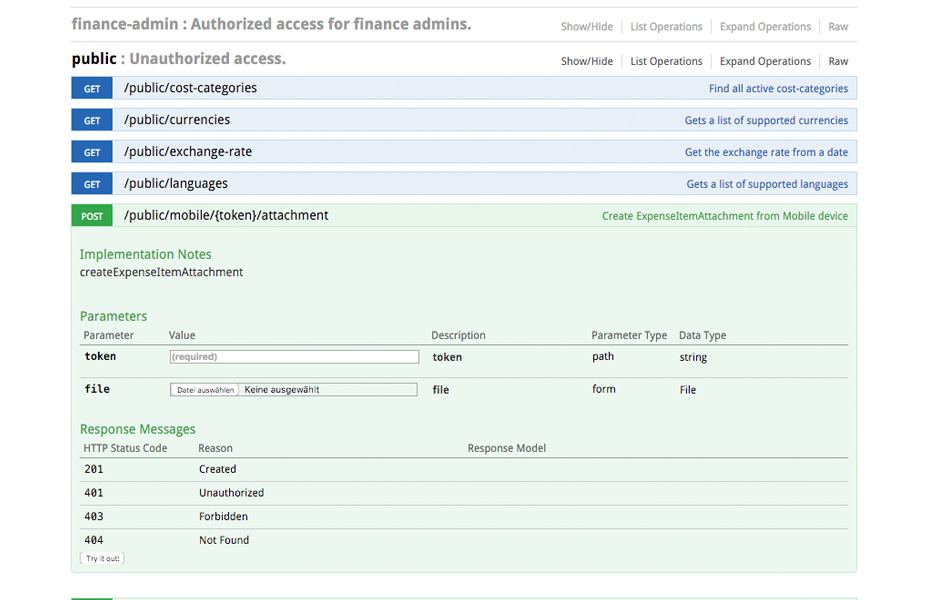
\includegraphics[width=0.80\textwidth]{swagger01}}
    \caption{Swagger: Reimbursement GUI}
    \label{fig:swagger01}
\end{figure}

\subsection{Frontend}

\subsubsection{AngularJS}
The tool uses the AngularJS framework for the client. Its data bindings and dependency injections reduces the amount of code need to be written. Further it uses HTML templates and a routing framework to create an interactive GUI. AngularJS is based on an MVC approach and is easy to integrate with REST services. \cite{angular}   

\subsubsection{Bootstrap}
Bootstrap is a framework that consists of HTML, CSS and JavaScript elements that can be used to create appealing responsive websites. It is supported by most of the desktop and mobile web browsers available. The tool uses Bootstrap v. 3.3.5. \cite{bootstrap}

\subsubsection{Bower}
The tool uses Bower for the client-side package management. Bower is a package manager for JavaScript web applications like AngularJS. It keeps track of the used assets, frameworks, libraries, etc. \cite{bower}  

\subsubsection{Grunt}
Grunt is a JavaScript task runner. We use it for our client-side build. Its plugin directory supports a lot of modules to optimize the development workflow. Code-uglifying, concating, sass-compiling, file operations, autoprefixing etc. \cite{grunt} 

